% \documentclass[11pt]{article}
% \usepackage[utf8]{inputenc}	% Para caracteres en español
% \usepackage{amsmath,amsthm,amsfonts,amssymb,amscd}
% \usepackage{multirow,booktabs}
% \usepackage[table]{xcolor}
% \usepackage{fullpage}
% \usepackage{lastpage}
% \usepackage{enumitem}
% \usepackage{fancyhdr}
% \usepackage{mathrsfs}
% \usepackage{wrapfig}
% \usepackage{setspace}
% \usepackage{calc}
% \usepackage{multicol}
% \usepackage{cancel}
% \usepackage[retainorgcmds]{IEEEtrantools}
% \usepackage[margin=3cm]{geometry}
% \usepackage{amsmath}
% \newlength{\tabcont}
% \setlength{\parindent}{0.0in}
% \setlength{\parskip}{0.05in}
% \usepackage{empheq}
% \usepackage{framed}
% \usepackage[most]{tcolorbox}
% \usepackage{xcolor}
% \colorlet{shadecolor}{orange!15}
% \geometry{margin=1in, headsep=0.25in}

\documentclass[11pt]{article}
 
\usepackage[margin=1in]{geometry} 
\usepackage{amsmath,amsthm,amssymb,scrextend}
\usepackage{fancyhdr}
\usepackage{graphicx}
\setlength{\headheight}{14pt}
\usepackage{xcolor}
\usepackage{color,soul}
\pagestyle{fancy}


\begin{document}
 
% --------------------------------------------------------------
%                         Start here
% --------------------------------------------------------------

\lhead{EE267 Virtual Reality}
\chead{Homework 2 Answers}
\rhead{Bohan Li}

\section{Theoretical Part}
\subsection{Simple Scanline Interpolation}
\subsubsection*{(i) Vertices in view space}
First, do the interpolation in y direction. For point ``m'' and ``n'' respectively:
\begin{align}
    A^{(m)} &= \frac{y - y_2}{y_1 - y_2}A_1 + \frac{y_1 - y}{y_1 - y_2}A_2,\\
    A^{(n)} &= \frac{y - y_2}{y_3 - y_2}A_3 + \frac{y_3 - y}{y_3 - y_2}A_2.
\end{align}

Then do the interpolation on the x axis using the information given by ``m'' and ``n'':
\begin{align}
    A^{(p)} &= \frac{x - x_n}{x_m - x_n}A^{(m)} + \frac{x_m - x}{x_m - x_n}A^{(n)}. 
\end{align}

\subsection{Phong Lighting}
First, we need to invert the window space coordinates to ndc coordinates. This is done using the viewport transform:
\begin{align*}
    x_{window} &= \frac{width}{2}(x_{ndc}+1)+x_{LL},\\
    y_{window} &= \frac{height}{2}(y_{ndc}+1)+y_{LL},\\
    z_{window} &= z_{ndc}/2 + 1/2.
\end{align*}
Therefore, the three points in ndc coordinates are given as: \[v_{1,ndc} = (-0.5,\ 0.333,\ 0.4\ ),\ v_{2,ndc} = (-0.833,\ -0.667,\ 0.0\ ),\ v_{3,ndc} = (0.5,\ -0.883,\ -0.4\ ).\]
From the given parameters of the perspective projection, the projection matrix (symmetric perspective) can be specified. Using the projection matrix, the forth element of clip space coordinate can be speficied as:
\begin{equation}
    w_{clip} = \frac{T_2}{z_{ndc}-\frac{T_1}{E_1}} = \frac{-\frac{22}{5}}{z_{ndc} - \frac{6}{5}},
\end{equation}
from which we can find the $w_{clip}$ coordinates for the three points as: \[w_{1,clip}= 5.5,\ w_{2,clip}= 3.67,\ w_{3,clip}= 2.75.\]
Therefore, the clip space coordinates are given as:
\[v_{1,clip} = (-2.2,\ 3.3,\ 2.2,\ 5.5),\ v_{2,clip} = (-2.936,\ -2.202,\ 0.0,\ 3.67),\ v_{3,clip} = (2.2,\ -2.2,\ -1.1,\ 2.75).\]
Finally, we can revert to the view space, which is done by multiplying by the invert of the projection matrix $v_{view} = M_{proj}^{-1}\ v_{clip}$ with the projection matrix given as:
\begin{equation*}
    M_{proj} = \begin{pmatrix}
        1 & 0 & 0 & 0\\[2pt]
        0 & 1 & 0 & 0\\[2pt]
        0 & 0 & -\frac{6}{5} & -\frac{22}{5}\\[2pt]
        0 & 0 & -1 & 0
    \end{pmatrix}.
\end{equation*}
Therefore, the view space coordinates:
\textcolor{blue}{\[v_{1,view} = (-2.75,\ 1.83,\ -5.5,\ 1),\ v_{2,view} = (-3.06,\ -2.44,\ -3.67,\ 1),\ v_{3,clip} = (1.38,\ -2.29,\ -2.75,\ 1).\]}

\subsubsection*{(ii) Color computation -- Phong shading}
In general, the color at a point is given as:
\begin{equation*}
    \text{color}_{RGB} = \frac{1}{k_c + k_l d + k_q d^2}(m_\text{RGB}^\text{diffuse} \cdot l_\text{RGB}^\text{diffuse} \cdot \max(L\cdot N,\ 0)),
\end{equation*}
where $L = \frac{l-v}{|l-v|}$ is the normalized vector from certain vertex to the light source, $N$ is the normalized surface normal vector. Therefore for the three vertices, the RGB colors are given by: 
\begin{align}
    \text{RGB}_1 &= (0.0018,\ 0,\ 0)\\
    \text{RGB}_2 &= (0,\ 0,\ 0)\\
    \text{RGB}_3 &= (0,\ 0,\ 0.0010).
\end{align}

The Mathematica code for such calculation can be found below: 
\begin{figure}[h!t]
    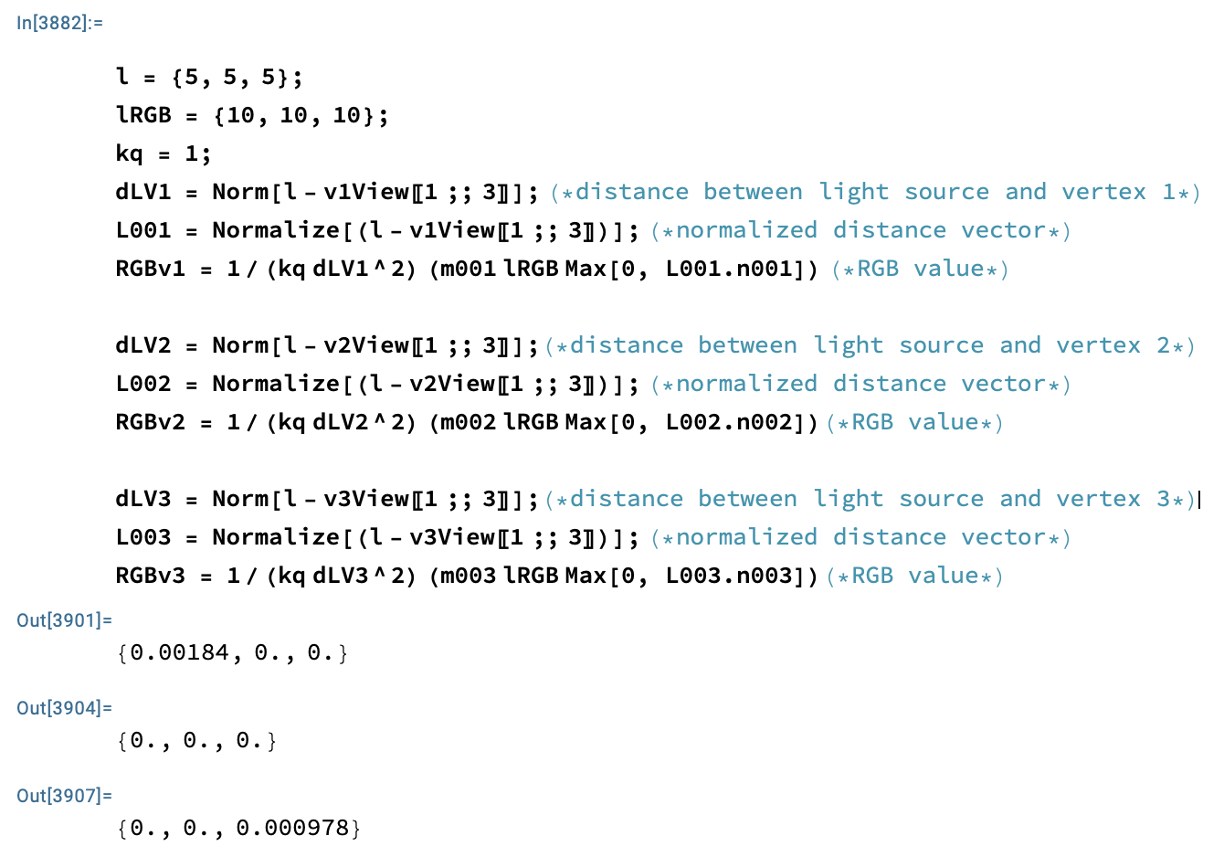
\includegraphics[width=0.8\textwidth]{figures/q1p2.png}
\end{figure}

In addition, I've also calculated the RGB color of each fragment inside the triangle. For Phong shading, the light calculation has to be carried out for each interpolated point separately. The objects needed to be interpolated are: the material properties, the normal vectors. Both the material diffuse property and the normal vector are in the form of length 3 vector, and the interpolation rule is exactly the same as written in previous derivations for color interpolation. Therefore, the properties of the interpolated points, including the position vectors, distance to the light source, material diffuse properties, normal vectors, and at last the RGB colors, are given in the table below as a summary.  

\begin{center}
    \begin{tabular}{ c c c c c c } 
    \hline
    ndc coord & 3D position & $d$ & $m_\text{RGB}^\text{diffuse}$ & $N$ & RGB \\[4pt] 
    \hline
    (2,3) & (-1.96, 0.58, -4.77) & 12.8 & (0.70, 0.10, 0.20) & (-0.68, 0.46, 0.57) &    (0.0095, 0.0016, 0.0027) \\ 
    (1,2) & (-2.77, -0.98, -4.26) & 13.5 & (0.34, 0.62, 0.04) & (-0.84, -0.29, 0.46) &  (0.0,0.0,0.0) \\ 
    (2,2) & (-1.70, -0.78, -4.11) & 12.7 & (0.38, 0.34, 0.28) & (-0.62, -0.34, 0.71) &  (0.0006, 0.0005, 0.0004) \\ 
    (3,2) & (-0.62, -0.57, -3.96) & 12.0 & (0.42, 0.06, 0.52) & (0.08, -0.30, 0.95) &   (0.018,0.0025,0.022) \\
    (1,1) & (-2.52, -2.34, -3.6) & 13.6 & (0.02, 0.86, 0.12) & (-0.58, -0.73, 0.38) &   (0.0,0.0,0.0) \\
    (2,1) & (-1.44, -2.13, -3.45) & 12.8 & (0.06, 0.58, 0.36) & (-0.27, -0.84, 0.48) &  (0.0,0.0,0.0) \\
    (3,1) & (0.37, -1.92, -3.3) & 12.1 & (0.10, 0.30, 0.60) & (0.21, -0.83, 0.52) &     (0.0,0.0,0.0) \\
    (4,1) & (0.71, -1.72, -3.15) & 11.4 & (0.14, 0.02, 0.84) & (0.61, -0.65, 0.45) &    (0.0,0.0,0.0) \\
    \hline
    \end{tabular}
\end{center}


\subsubsection*{(iii) Shader Speed}
The case where per-vertex shading involves more calculation could be: when the lighting condition is complex (the lighting calculation is extremely time-consuming), and the triangles are sufficiently fine. For instance, each triangle will only contains 1 grid point inside it. In such case, the number of fragment calculation per triangle is 1, meaning that the lighting calculation needs to be carried out 1 time. While for per-vertex calculation involves lighting calculation 3 times per triangle, which consumes more time.

\newpage

\section{Programming Part}
\subsubsection*{2.1.1.3 Attenuation Factor Observations}
The influence of the attenuation factor $k_q$ can be observed in the following figure. Without attenuation, the point light source can generate equal amount of brightness on each teapot. When there is attenuation, the teapot farther away from the point light source can be dimmer. 
\begin{figure}[h!t]
    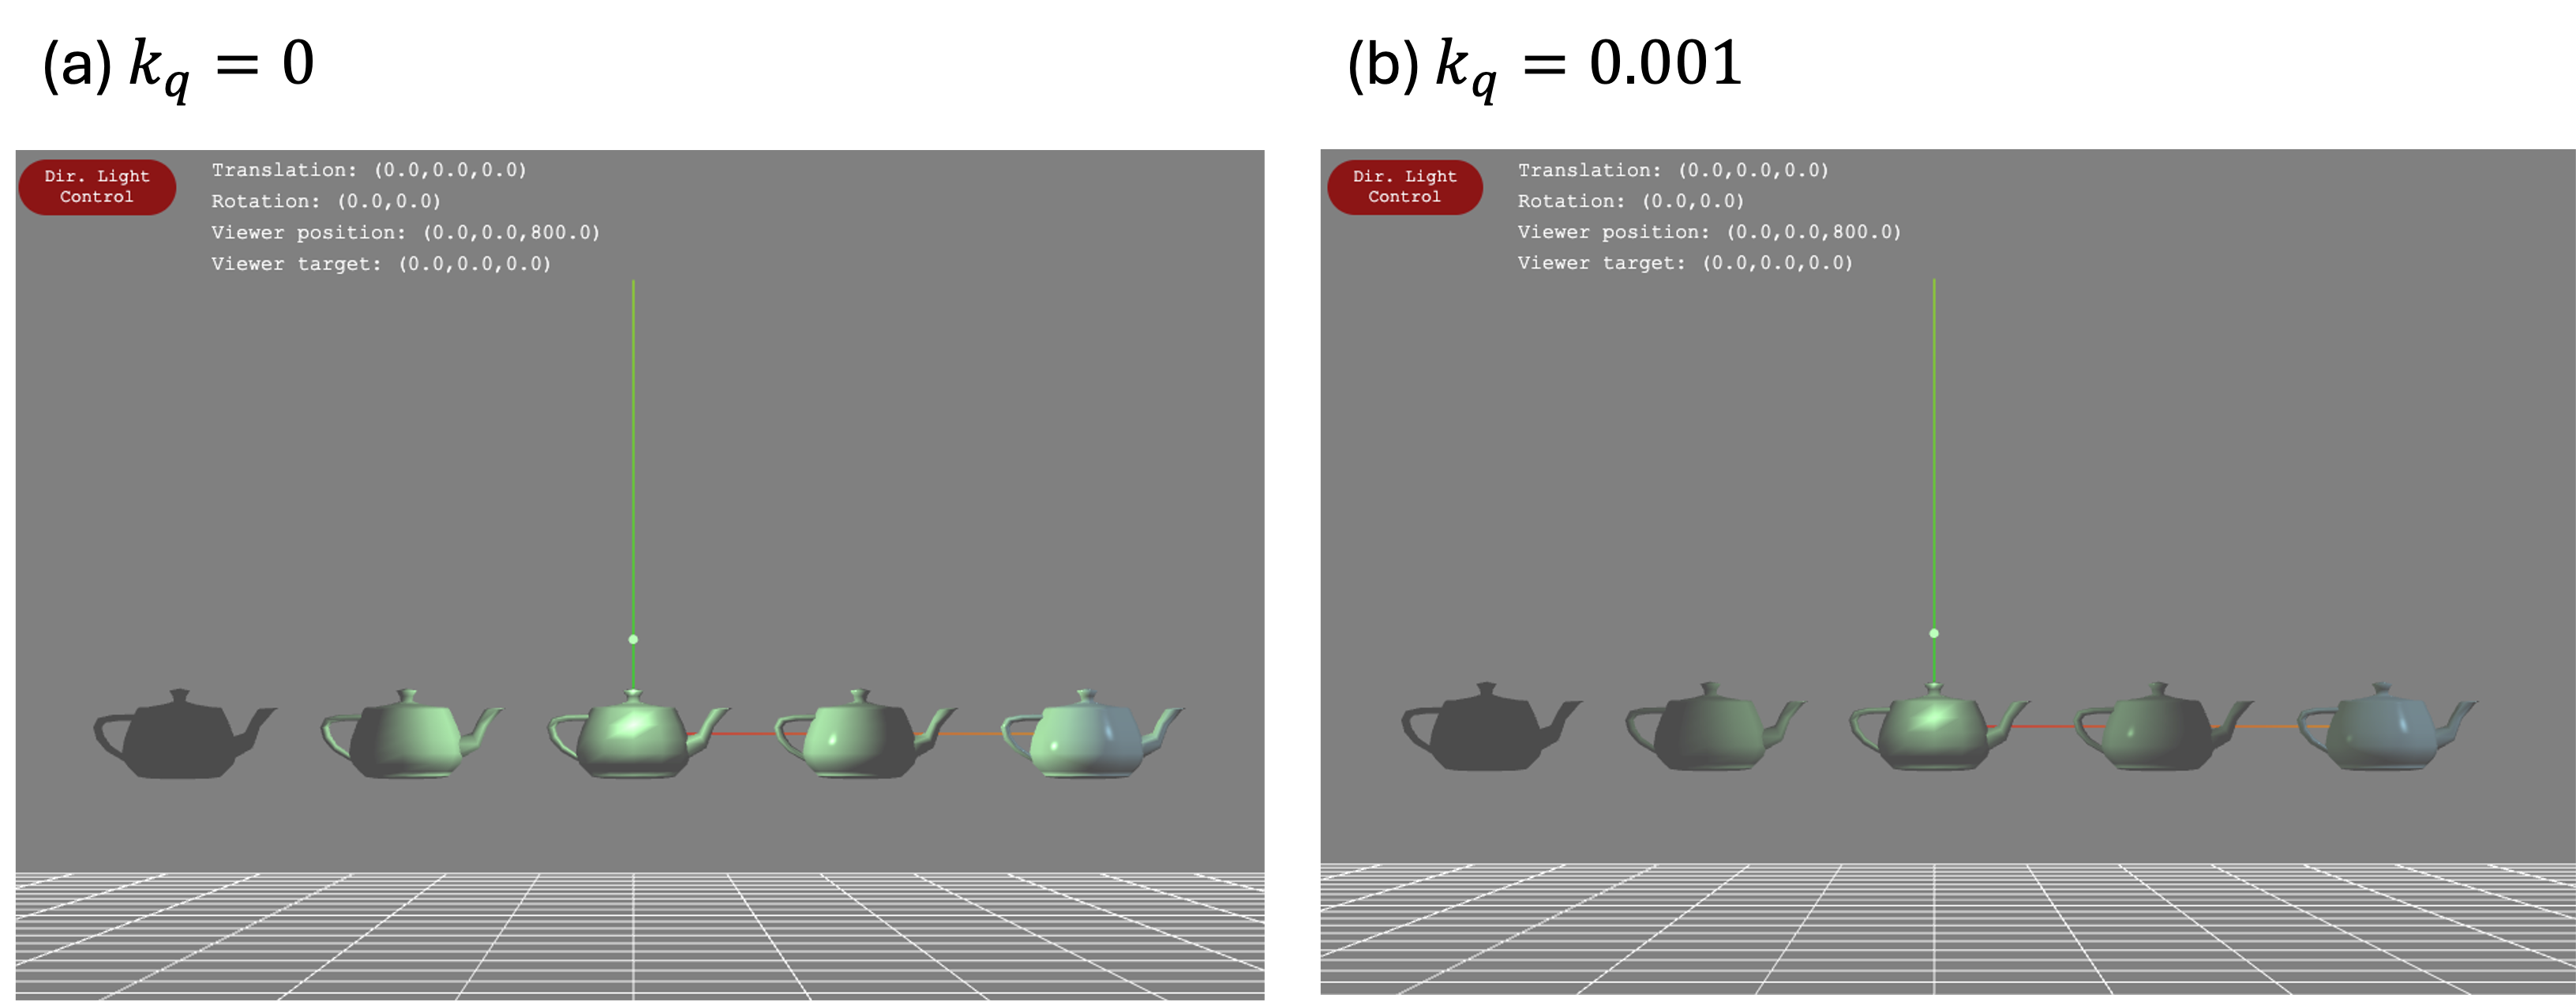
\includegraphics[width=\textwidth]{figures/2p1p1p3.png}
\end{figure}

\subsubsection*{2.2.2.1 Gouraud vs Phong Shading Comparison}
As can be observed in the figure above, Gouraud shading gives more coarse rendering results while Phong shading is finer. This is especially true for specular reflection, where the reflection bright spot can be spatially detailed. So such is the advantage of Phong shading, to generate more realistic and finer rendering results. On the other hand, the downside of Phong shading is the computational speed, as the lighting computations are carried out for each fragments. The Gouraud shading can be much faster in speed.  


\end{document}